\documentclass[9pt,twocolumn,twoside]{pnas-new}
%\documentclass[9pt,twocolumn,pnasresearcharticle]{pnas-new}
%\documentclass[9pt,twocolumn,twoside]{pnas-new}
% Use the lineno option to display guide line numbers if required.

%%%%% NEW MATH DEFINITIONS %%%%%
\usepackage{amsmath,bbm,bm}
\usepackage{amssymb}
\usepackage{amsfonts}
\usepackage{amsthm}
\usepackage{mathtools}

% commands
% global count (no section number)
\newtheorem{thm}{Theorem}%[section]
\newtheorem{lem}{Lemma}
\newtheorem{prop}{Proposition}
\newtheorem{cor}{Corollary}
\newtheorem{conj}{Conjecture}
\newtheorem{aspt}{Assumption}
\newtheorem{claim}{Claim}
\newtheorem{rmk}{Remark}
\newtheorem{commt}{Comment}
\newtheorem{defn}{Definition}

% algorithm
%\usepackage{algorithm, algorithmic}
%\usepackage{algorithm2e}
\usepackage{tabularx}
%\usepackage[table,xcdraw]{xcolor}

% Comments
% \usepackage{xcolor} % already loaded
\newcount\comments  % 0 suppresses notes to selves in text
\comments=1  % TODO: change to 0 for final version
\newcommand{\genComment}[2]{\ifnum\comments=1{\textcolor{#1}{\textsf{\footnotesize #2}}}\fi}
\newcommand{\ed}[1]{\genComment{red}{[EI:#1]}}
\newcommand{\giles}[1]{\genComment{green}{[GH:#1]}}
\newcommand{\kevin}[1]{\genComment{blue}{[KT:#1]}}


% Mark sections of captions for referring to divisions of figures
\newcommand{\figleft}{{\em (Left)}}
\newcommand{\figcenter}{{\em (Center)}}
\newcommand{\figright}{{\em (Right)}}
\newcommand{\figtop}{{\em (Top)}}
\newcommand{\figbottom}{{\em (Bottom)}}
\newcommand{\captiona}{{\em (a)}}
\newcommand{\captionb}{{\em (b)}}
\newcommand{\captionc}{{\em (c)}}
\newcommand{\captiond}{{\em (d)}}


\newcommand\seq[2]{{#1}\!:\!{#2}}
\newcommand\R{\mathbb{R}}
\newcommand\Var{\mathrm{Var}}
\newcommand\var{\Var}
\newcommand\Cov{\mathrm{Cov}}
\newcommand\cov{\Cov}
\newcommand\iid{\mathrm{iid}}
\newcommand\dist{d}
\newcommand\lik{\mathcal{L}}
\newcommand\prob{\mathbb{P}}
\newcommand\E{\mathbb{E}}
\newcommand\loglik{\ell}
\newcommand\process{\texttt{process}}
\newcommand\dimtheta{\mathrm{dim}_{\Theta}}
\newcommand\param{\,;}
\newcommand\giventh\param
\newcommand\given{{\,\vert\,}}
\newcommand\code[1]{\texttt{#1}}
\newcommand\ceil[1]{\lceil #1 \rceil}
\newcommand\floor[1]{\lfloor #1 \rfloor}
\newcommand\1{\bm{1}}


% Highlight a newly defined term
\newcommand{\newterm}[1]{{\bf #1}}


% Figure reference, lower-case.
\def\figref#1{figure~\ref{#1}}
% Figure reference, capital. For start of sentence
\def\Figref#1{Figure~\ref{#1}}
\def\twofigref#1#2{figures \ref{#1} and \ref{#2}}
\def\quadfigref#1#2#3#4{figures \ref{#1}, \ref{#2}, \ref{#3} and \ref{#4}}
% Section reference, lower-case.
\def\secref#1{section~\ref{#1}}
% Section reference, capital.
\def\Secref#1{Section~\ref{#1}}
% Reference to two sections.
\def\twosecrefs#1#2{sections \ref{#1} and \ref{#2}}
% Reference to three sections.
\def\secrefs#1#2#3{sections \ref{#1}, \ref{#2} and \ref{#3}}
% Reference to an equation, lower-case.
\def\eqref#1{equation~\ref{#1}}
% Reference to an equation, upper case
\def\Eqref#1{Equation~\ref{#1}}
% A raw reference to an equation---avoid using if possible
\def\plaineqref#1{\ref{#1}}
% Reference to a chapter, lower-case.
\def\chapref#1{chapter~\ref{#1}}
% Reference to an equation, upper case.
\def\Chapref#1{Chapter~\ref{#1}}
% Reference to a range of chapters
\def\rangechapref#1#2{chapters\ref{#1}--\ref{#2}}
% % Reference to an algorithm, lower-case.
% \def\algref#1{algorithm~\ref{#1}}
% % Reference to an algorithm, upper case.
% \def\Algref#1{Algorithm~\ref{#1}}
% \def\twoalgref#1#2{algorithms \ref{#1} and \ref{#2}}
% \def\Twoalgref#1#2{Algorithms \ref{#1} and \ref{#2}}
% Reference to a part, lower case
\def\partref#1{part~\ref{#1}}
% Reference to a part, upper case
\def\Partref#1{Part~\ref{#1}}
\def\twopartref#1#2{parts \ref{#1} and \ref{#2}}

\def\eps{{\epsilon}}

\def\gN{{\mathcal{N}}}
\def\gX{{\mathcal{X}}}
\def\gY{{\mathcal{Y}}}


\makeatletter
\newcommand*{\addFileDependency}[1]{% argument=file name and extension
\typeout{(#1)}% latexmk will find this if $recorder=0
% however, in that case, it will ignore #1 if it is a .aux or 
% .pdf file etc and it exists! If it doesn't exist, it will appear 
% in the list of dependents regardless)
%
% Write the following if you want it to appear in \listfiles 
% --- although not really necessary and latexmk doesn't use this
%
\@addtofilelist{#1}
%
% latexmk will find this message if #1 doesn't exist (yet)
\IfFileExists{#1}{}{\typeout{No file #1.}}
}\makeatother

\newcommand*{\myexternaldocument}[1]{%
\externaldocument{#1}%
\addFileDependency{#1.tex}%
\addFileDependency{#1.aux}%
}

\usepackage{tabto}



\templatetype{pnasresearcharticle} % Choose template
% {pnasresearcharticle} = Template for a two-column research article
% {pnasmathematics} %= Template for a one-column mathematics article
% {pnasinvited} %= Template for a PNAS invited submission

\begin{document}

\title{Accelerated Inference for Partially Observed Stochastic Processes with Automatic Differentiation}

% Use letters for affiliations, numbers to show equal authorship (if applicable) and to indicate the corresponding author
\author[a]{Kevin Tan}
\author[a]{Giles Hooker}
\author[b,1]{Edward L. Ionides}
%\author[a]{Author Three}

\affil[a]{University of Pennsylvania}
\affil[b]{University of Michigan}
%\affil[c]{Affiliation Three}

% Please give the surname of the lead author for the running footer
\leadauthor{Tan}

% Please add a significance statement to explain the relevance of your work
\significancestatement{Many scientific models involve highly nonlinear stochastic dynamical systems which can be observed only via noisy and incomplete measurements. Prior to this work, iterated filtering algorithms were the only class of algorithms for maximum likelihood estimation that did not require access to the system's transition probabilities, instead needing only a simulator of the system dynamics. We leverage recent advances in automatic differentiation to propose a hybrid algorithm that requires only a differentiable simulator for maximum likelihood estimation. Our new method outperforms previous approaches on a challenging problem in epidemiology.}

% Please include corresponding author, author contribution and author declaration information
\authorcontributions{K.T. and E.L.I. designed research; K.T. analyzed data; K.T., G.H. and E.L.I. performed research, K.T., G.H., and E.L.I. wrote the manuscript.}
\authordeclaration{The authors declare no competing interests.}
\correspondingauthor{\textsuperscript{1}To whom correspondence should be addressed. E-mail: kevtan@wharton.upenn.edu}

% At least three keywords are required at submission. Please provide three to five keywords, separated by the pipe symbol.
\keywords{Sequential Monte Carlo $|$ Automatic Differentiation $|$ Particle Filter $|$ Markov Process $|$ Maximum Likelihood}

\begin{abstract}
  Automatic differentiation (AD) has driven recent advances in machine learning, including deep neural networks and Hamiltonian Markov Chain Monte Carlo methods. Partially observed nonlinear stochastic dynamical systems have proved resistant to AD techniques as widely used particle filter algorithms yield a likelihood function that is discontinuous as a function of the model parameters. Furthermore, most approaches are not compatible with the desire for simulation-based inference without access to the system's transition probabilities. We propose a new representation that embeds existing methods in a theoretical framework that readily permits extension to a new class of algorithms, providing opportunities for optimizing a bias/variance tradeoff. Further, we develop optimization algorithms suited to the Monte Carlo properties of the derivative estimate, including a hybrid algorithm that requires only a differentiable simulator for maximum likelihood estimation. Promising numerical results indicate that a hybrid algorithm that uses AD to refine a coarse solution from iterated filtering can beat current state-of-the-art methods on a challenging scientific benchmark problem.
\end{abstract}

\dates{This manuscript was compiled on \today}
\doi{\url{www.pnas.org/cgi/doi/10.1073/pnas.XXXXXXXXXX}}


\maketitle
\thispagestyle{firststyle}
\ifthenelse{\boolean{shortarticle}}{\ifthenelse{\boolean{singlecolumn}}{\abscontentformatted}{\abscontent}}{}

\firstpage{5}
% Use \firstpage to indicate which paragraph and line will start the second page and subsequent formatting. In this example, there are a total of 11 paragraphs on the first page, counting the first level heading as a paragraph. The value {12} represents the number of the paragraph starting the second page. If a paragraph runs over onto the second page, include a bracket with the paragraph line number starting the second page, followed by the paragraph number in curly brackets, e.g. "\firstpage[4]{11}".


% If your first paragraph (i.e. with the \dropcap) contains a list environment (quote, quotation, theorem, definition, enumerate, itemize...), the line after the list may have some extra indentation. If this is the case, add \parshape=0 to the end of the list environment.
\dropcap{M}any scientific models involve highly nonlinear stochastic dynamic systems, where there may be significant uncertainty in both the process dynamics and the measurements of the system. Despite the ubiquity of such partially observed stochastic processes with the Markov property (also known as, continuous-state continuous-time hidden Markov models (HMMs), partially-observed Markov processes (POMPs), or partially-observed stochastic nonlinear dynamical systems) in fields as diverse as epidemiology \cite{he10, stocks17}, ecology \cite{knape12}, and finance \cite{kim08, breto14}, estimation and inference within this class of models is a difficult problem with several challenges. 

Popular methods for estimation and inference in these scenarios (such as the EM algorithm, the various Kalman filter variants, and MCMC) either struggle with complex models that have intractable likelihood functions, or assume access to state transition densities. This is a problem in some critical applications, such as disease modeling, where transition densities are unavailable. However, in such cases a simulator may be readily available. In this case, the particle filter with the bootstrap proposal, a popular method for solving the filtering problem in partially-observed dynamical systems, provides an unbiased estimate of the likelihood \cite{delmoral2004feynman} without requiring evaluation of the transition density of the latent Markov process, enabling an arbitrary model simulator to be plugged into the algorithm. 

A series of related algorithms \cite{welch2009abc, wood2010sl, doucet2010pmcmc, ionides08, ionides15} enable parameter estimation within these models. In particular, the improved iterated filtering algorithm (IF2) \cite{ionides15} is the only simulation-based full-information maximum likelihood method available, whereas particle MCMC \cite{doucet2010pmcmc} and $\text{SMC}^2$ \cite{chopin13} are the only simulation-based full-information Bayesian methods available in the literature thus far. However, accurate parameter estimation with significant Monte-Carlo noise in the likelihood estimate is challenging, especially when the Monte Carlo variance of the evaluation is high and the number of parameters is not small. For example, though in practice the algorithm of Ionides et al. \cite{ionides15} converges quickly to a neighborhood of the MLE, it often struggles to successfully optimize the last few-units of the log-likelihood. This necessitates a new approach.


\subsection{Automatic Differentiation for Particle Filters}

Recent advances in automatic differentiation (AD) for particle filters \cite{blei2018vsmc, jon2018diffpf, corenflos21, scibior2021dpf, doucet2022particlebased} have drawn attention to AD as a tool for inference in partially observed stochastic processes. However, existing approaches are either asymptotically biased \cite{blei2018vsmc, jon2018diffpf}, have high variance \cite{poyiadjis11, scibior21}, computationally expensive \cite{corenflos21, chen24}, or need access to transition densities \cite{poyiadjis11, scibior21, doucet2022particlebased, chen24}.

In particular, Scibior and Wood \cite{scibior21} show that the estimators derived in Poyiadjis et al. \cite{poyiadjis11} can be attained with AD, through with a simple tweak (the "stop-gradient trick") to the particle filter that does not modify its likelihood estimates. However, their method is not fully compatible with simulation-based inference and the mathematical motivation behind the stop-gradient trick is not apparent. 

%We show that another simple tweak enables this compatibility and corresponds to a special case of our MOP-$\alpha$ algorithm. 

\kevin{Can someone who's reading through the words and glazing through the math get the idea that (1) we're running AD on the PF, and (2) using an off-policy resampling trick to get our estimator. Should I hedge by writing the SI in Del Moral language? }

\subsection{Our Contributions}
We develop a new approach to statistical inference via AD for particle filters which addresses the above concerns. We construct a new theoretical framework that bypasses the paradox of differentiating through a Monte-Carlo algorithm with discontinuous resampling.

Our key observation is that one can turn this into a problem of differentiating through a series of smooth measurement density ratios and (through the reparametrization trick) a differentiable simulator. To do so, we construct a suitably reweighted family of particle filters that we call \textbf{Measurement Off-Policy-$\alpha$} (MOP-$\alpha$), for some $\alpha \in [0,1]$ that optimizes a bias-variance tradeoff. This family encompasses the biased gradient estimator of \cite{blei2018vsmc} when $\alpha=0$, and the high-variance gradient estimate from \cite{poyiadjis11, scibior21} when $\alpha=1$. It does not require access to the transition densities, and works with just a differentiable simulator.

We show that these off-policy particle filters successfully target the posterior, recover desirable gradient estimates previously encountered in the literature, and possess other desirable theoretical properties. We also derive a linear convergence rate for gradient methods on the particle filter in the presence of strong convexity, providing support for numerical optimization with AD for the particle filter. 

This allows us to develop improved algorithms for maximum likelihood/MAP estimation in highly nonlinear stochastic dynamical systems. We propose a hybrid algorithm called \textbf{Iterated Filtering with Automatic Differentiation (IFAD)} that warm-starts iterative first or second-order gradient methods with a coarse solution obtained from a few rounds of iterated filtering. Promising numerical results indicate that IFAD beats IF2 (and by the numerical results of \cite{ionides15}, also IF1 and the Liu-West filter \cite{liuwest01}) on a challenging problem in epidemiology, the Dhaka cholera model of \cite{king08}.

These improvements also extend to Bayesian inference, as we show that we can use the MOP-$\alpha$ gradient estimates within a No-U-Turn Sampler (NUTS) \cite{homan14} in conjunction with a nonparametric empirical Bayes-style prior estimated with IF2 to reduce the burn-in period of particle MCMC \cite{doucet2010pmcmc} from the $1.4 \times 10^6$ iterations in \cite{fasiolo16} to just $500$. 

\section{Problem Setup}

Consider an unobserved Markov process $(X_t)_{t \geq t_0}$, with observations $Y_1,...,Y_N$ realized at values $y_1^*,...,y_N^*$ at timesteps $t_1,..., t_N$. The process is parameterized by an unknown parameter $\theta \in \Theta \subseteq \R^p$, where the states $X_t$ take values in the state space $\gX \subseteq \R^d$, the observations $Y_n$ take values in $\gY,$ and we write $X_n := X_{t_n}$. 

% By a similar decomposition to that in \cite{doucet2009tutorial}, we find that the joint density of $X_{0:N}, Y_{1:N}$ can be factored as
% \begin{align*}
%     &f_{X_{0: N}, Y_{1: N}}\left(x_{0: N}, y_{1: N} ; \theta\right)\\
%     &=f_{X_0}\left(x_0 ; \theta\right) \prod_{n=1}^N f_{X_n \mid X_{n-1}}\left(x_n \mid x_{n-1} ; \theta\right) f_{Y_n \mid X_n}\left(y_n \mid x_n ; \theta\right).
% \end{align*}

We write $f_{X_n|X_{n-1}}\left(x_{n} \mid x_{n-1}; \theta\right)$ for the process model, writing $\texttt{process}\left(x_n; \theta\right)$ for its corresponding simulator, $f_{Y_n|X_n}\left(y_n \mid x_n; \theta\right)$ the measurement model, and $y_n^*$ for the actual values of the observations that were observed. We call $f_{X_{1:n}|Y_{1:n}}(x_{1:n}|y_{1:n}^*; \theta)$ the posterior distribution of states, and $f_{X_{n}|Y_{1:n}}(x_n|y_{1:n}^*; \theta)$ the filtering distribution at time $t_n$. Superscripts $x_{n,j}^A$ denote the ancestral trajectory of particle $j$ at time $n$, and $a(\cdot)$ is the ancestor function. For simplicity, we omit the dependence of the likelihood and other suitable calculations on $X_0.$ 

The above are defined on a probability space $(\Omega, \Sigma, \prob).$ 
To maintain an algorithmic and practical interpretation of our theory, we identify the seed with an element of the sample space $\omega \in \Omega$, as a random seed determines the entire sequence of pseudo-random numbers as generated by a computer. 

%When two algorithms share the same seed, this corresponds to the method of common random numbers. 


\section{Off-Policy Particle Filters}

As mentioned earlier, instead of directly differentiating through a particle filter, one can instead differentiate through the simulator and measurement densities. We construct an algorithm called \textbf{Measurement Off-Policy-$\alpha$} (MOP-$\alpha$) that targets the posterior (i.e. almost sure convergence of every measurable bounded functional of particles to its expectation under the posterior) and likelihood, and whose gradient yields a score estimate encompassing those of \cite{poyiadjis11, scibior21, blei2018vsmc}.


\begin{algorithm}[H]
	\caption{MOP-$\alpha$}
    \label{alg:mop}
	     \textbf{Input:} Number of particles $J$, timesteps $N$, measurement model $f_{Y_n|X_n}(y_n^*|x_n, \theta)$, simulator $\process(x_{n+1}|x_n, \theta)$, evaluation parameter $\theta$, behavior parameter $\phi$, seed $\omega$. \newline
        \textbf{If $\theta \neq \phi$:}
            Fix $\omega$, and filter at $\phi$ to obtain $X_{n,j}^{P,\phi}, X_{n,j}^{F,\phi}$. \newline
        \textbf{Else:} Fix $\omega$, and set $X_{n,j}^{P,\phi}, X_{n,j}^{F,\phi}$ to be copies of $X_{n,j}^{P,\theta}, X_{n,j}^{P,\theta}$. \newline
		\textbf{Initialize } particles ${X}_{0,j}^{F,\theta}\sim {f}_{{X}_{0}}\left(\cdot\giventh{\theta}\right)$, weights $w^{F,\theta}_{0,j}= 1$. \newline
		\textbf{For} $n=1,...,N$: \newline
            \hspace*{4mm} Accumulate discounted weights, $w_{n,j}^{P,\theta} = \big(w_{n-1,j}^{F,\theta}\big)^\alpha$.\newline
            \hspace*{4mm} Simulate process model,
            ${X}_{n,j}^{P,\theta}\sim {f}_{{X}_{n}|{X}_{n-1}}\big(\cdot|{X}_{n-1,j}^{F};{\theta}\big)$. \newline
            \hspace*{4mm} Measurement density,
            $g^{\theta}_{n,j}={f}_{{Y}_{n}|{X}_{n}}(y_{n}^{*}|{X}_{n,j}^{P,\theta}\giventh{\theta})$. \newline
            \hspace*{4mm} Compute $L_n^{B,\theta,\alpha} ={\sum_{j=1}^Jg^\theta_{n,j} w^{P,\theta}_{n,j}}/{\sum_{j=1}^J  w^{P,\theta}_{n,j}}$. \newline
            \hspace*{4mm} Conditional likelihood under $\phi$,
            $L_n^{\phi} = \frac{1}{J}\sum_{m=1}^{J}g^{\phi}_{n,m}$.\newline
            \hspace*{4mm} Select indices $k_{1:J}$ with $\prob\big(k_{j}=m\big) \propto g^{\phi}_{n,m}$. \newline
            \hspace*{4mm} Resample particles ${X}_{n,j}^{F,\phi}={X}_{n,k_{j}}^{P,\phi}$. \newline
            \hspace*{4mm} Resample corrected weights
            $w_{n,j}^{F,\theta}= w^{P,\theta}_{n,k_j}  { g^{\theta}_{n,k_j}}/{ g^{\phi}_{n,k_j}}$.\newline
            \hspace*{4mm} Compute $ L_n^{A,\theta,\alpha} = L_n^\phi\cdot {\sum_{j=1}^J w^{F,\theta}_{n,j}}/{\sum_{j=1}^J  w^{P,\theta}_{n,j}}$.\newline
		\textbf{Return:} likelihood estimate $\hat{\lik}(\theta) = \prod_{n=1}^N L_n^{A,\theta,\alpha}$ or $\hat{\lik}(\theta) = \prod_{n=1}^N L_n^{B,\theta,\alpha}$, filtering distributions $\{(X_{n,j}^{F, \theta}, w^{F,\theta}_{n,j})\}_{n,j=1}^{N,J}.$
\end{algorithm}


\subsection{Algorithm Outline} 
We obtain two coupled sets of particles, one under $\phi \in \Theta$, and another with the process model at $\theta \in \Theta$ but the resampling indices from the run at $\phi$ (hence the "off-policy" moniker). If $\theta$ and $\phi$ coincide, one only needs one particle filter run at $\theta=\phi$, otherwise one needs two runs at the same seed $\omega \in \Omega$.

We can then reweight the conditional likelihoods by a correction factor accumulated over time to account for the resampling under $\phi$. That is, writing $g^{\theta}_{n,j}={f}_{{Y}_{n}|{X}_{n}}(y_{n}^{*}|{X}_{n,j}^{P,\theta}\giventh{\theta})$ for the measurement density, $L_n^{\phi} = \frac{1}{J}\sum_{m=1}^{J}g^{\phi}_{n,m}$ for the conditional likelihood estimate under $\phi$, and $k_j \sim \text{Categorical}(g^{\phi}_{n,1},...,g^{\phi}_{n,J})$ for the resampling indices under $\phi$, we can estimate the conditional likelihood under $\theta$ as
\vspace*{-2.5mm}
\begin{equation}
     \label{eq:mop-conditional-likelihood}
     L_n^{B,\theta,\alpha} = \frac{\sum_{j=1}^Jg^\theta_{n,j} w^{P,\theta}_{n,j}}{\sum_{j=1}^J  w^{P,\theta}_{n,j}} \text{ or } L_n^{A,\theta,\alpha} = L_n^\phi\cdot \frac{\sum_{j=1}^J w^{F,\theta}_{n,j}}{\sum_{j=1}^J  w^{P,\theta}_{n,j}},
     \vspace*{-2.5mm}
\end{equation}
recursively weighting each particle by 
\vspace*{-2.5mm}
\begin{equation}
    \label{eq:weighting-scheme}
    w_{n,j}^{P,\theta} = (w_{n-1,j}^{F,\theta})^\alpha,  w^{F,\theta}_{n,j} = w^{P,\theta}_{n,k_j} { g^{\theta}_{n,k_j}}/{ g^{\phi}_{n,k_j}}, w^{F,\theta}_{0,j}= 1.
    \vspace*{-2.5mm}
\end{equation}

The before-resampling conditional likelihood estimate $L_n^{B,\theta,\alpha}$ should be used in general, as it has slightly lower variance than the after-resampling estimate $L_n^{A,\theta,\alpha}$, but the latter is useful in deriving properties of the MOP-$\alpha$ gradient estimate such as that in Theorem \ref{thm:mop-functional-forms}.

This yields a suitably reweighted particle filter that targets the posterior under $\theta$ and produces a strongly consistent likelihood estimate for the likelihood at $\theta$. Taking the gradient with respect to $\theta$ of the estimate for the log-likelihood at $\theta$ then yields an estimate for the score at $\theta$. 




\subsection{Discounting Weights for a Bias-Variance Tradeoff}

As mentioned earlier, the correction factors accumulate over time. If $\theta$ and $\phi$ coincide, one can discount the correction factors from previous timesteps by some $\alpha \in [0,1]$, as seen in Equation \ref{eq:weighting-scheme}, while still targeting the posterior and likelihood at $\theta$. This lets us optimize a bias-variance tradeoff for the MOP-$\alpha$ score estimate. When $\alpha=1$, MOP-$1$ maintains the memory of each particle's ancestral trajectory, recovering the consistent but high-variance gradient estimate from \cite{poyiadjis11, scibior21}. When $\alpha=0$, MOP-$0$ considers only single-step transition dynamics, recovering the low-variance but asymptotically biased gradient estimator of \cite{blei2018vsmc}. 


\subsection{MOP-$\alpha$ Encompasses the Estimators of \cite{poyiadjis11, scibior21, blei2018vsmc}}

\cite{scibior21} show that the estimate of \cite{blei2018vsmc} is the gradient of a vanilla particle filter when resampling terms are dropped, and also recover the estimate of \cite{poyiadjis11} through applying a ``stop-gradient trick" to the particle filter. It turns out that both of these, when applied on the bootstrap filter, correspond to special cases of MOP-$\alpha$.


$\alpha$ therefore controls an exponentially-weighted moving average, determining how much "memory" the resulting gradient estimate has over ancestral trajectories. This is illustrated in Figure \ref{fig:biasvar}, in the context of the Dhaka cholera model of \cite{king08}. 

\begin{thm}[MOP-$0$ and MOP-$1$ Functional Forms]
    \label{thm:mop-functional-forms}
    Write $\nabla_\theta \hat\ell^\alpha(\theta)$ for the gradient estimate yielded by MOP-$\alpha$ when $\theta=\phi$ and we use the after-resampling conditional likelihood estimate so that $\hat\lik(\theta) = \prod_{n=1}^N L_n^{A, \theta, \alpha}$. Then, when $\alpha=0$,
    \vspace*{-2.5mm}
    \begin{equation}
        \nabla_\theta \hat\ell^0(\theta) 
        = \frac{1}{J} \sum_{n=1}^N \sum_{j=1}^J \nabla_\theta \log\left(f_{Y_n|X_{n}}(y_n^*|x_{n,j}^{F, \theta}; \theta)\right),
        \vspace*{-2.5mm}
    \end{equation}
    yielding \cite{blei2018vsmc} on the bootstrap filter. When $\alpha=1$,
    \vspace*{-2.5mm}
    \begin{equation}
        \nabla_\theta \hat{\ell}^1(\theta) 
        = \frac{1}{J}\sum_{j=1}^J \nabla_\theta \log f_{Y_{1:N}|X_{1:N}}\left(y_{1:N}^* | x_{1:n,j}^{A, F,\theta}\right),
    \vspace*{-2.5mm}
    \end{equation}
    yielding the estimator of \cite{poyiadjis11, scibior21} with the bootstrap filter.
\end{thm}

We defer the proof to the supplementary material. It relies on a useful decomposition of the after-resampling conditional likelihood estimate $L_n^{A,\theta,\alpha}$ that yields a telescoping product in the MOP-$1$ case. Repeated applications of the log-derivative identity that $\nabla_x \log(f(x)) = (\nabla_x f(x))/f(x)$, and noting that when $\theta=\phi$, that $w_{n,j}^{P,\theta}$ evaluates to $1$, yield the result. 

This further illustrates how $\alpha$ dictates the "memory" of the gradient estimate. As \cite{scibior2021dpf} remark, the MOP-$0$ estimator of \cite{blei2018vsmc} only considers single-step quantities, and is "memoryless" beyond a single step. This is in contrast to the case when $\alpha=1,$ as that estimate of \cite{poyiadjis11} only considers the surviving particles at time $N$, fully tracking dependencies over time. 


\begin{figure}[ht!]
    \centering
    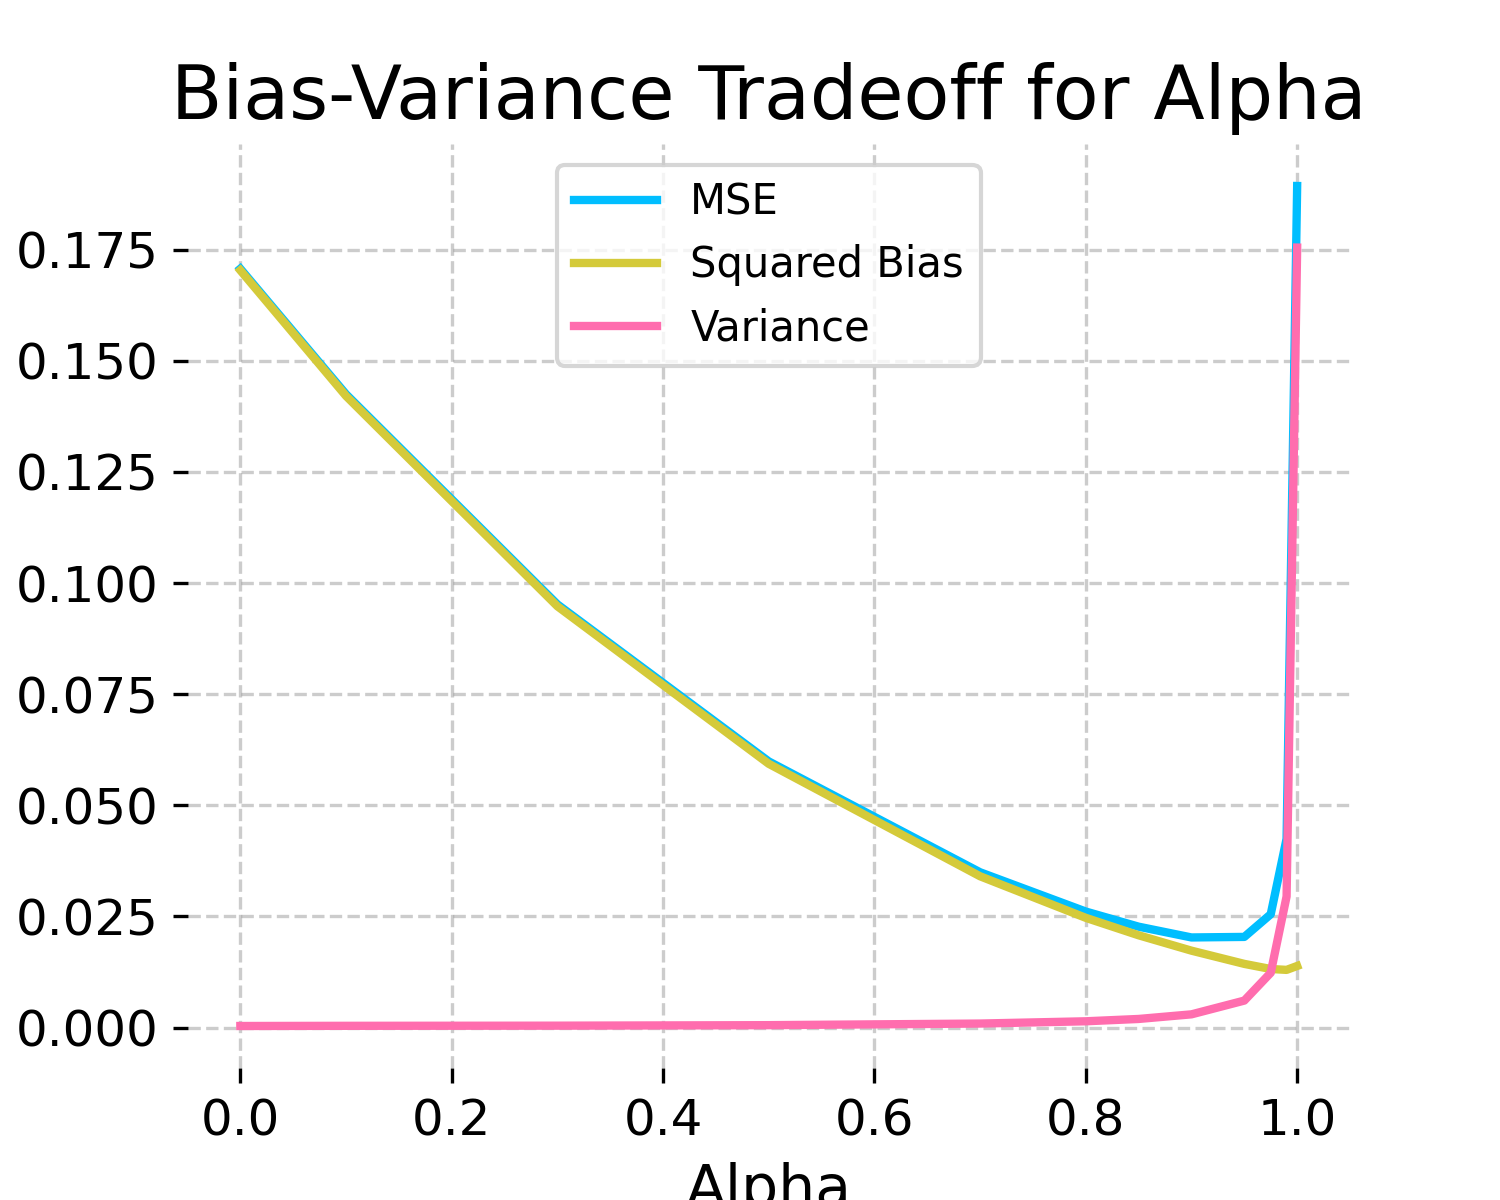
\includegraphics[width=\textwidth/3]{imgs/095/biasvar.png}
    \caption{Illustration of the bias-variance tradeoff induced by the discounting hyperparameter $\alpha$, on the Dhaka cholera model of \cite{king08}. We display the MSE of score estimates for the trend in transmission, evaluated at the MLE.}
    \label{fig:biasvar}
\end{figure}

\subsection{Summary of Theoretical Guarantees}

We bypass the issue of differentiating through a Monte Carlo algorithm with discontinuous resampling by turning it into a problem of differentiating through a simulator and a series of measurement density ratios. Although we defer the theoretical analysis of the resulting algorithm, MOP-$\alpha$, to Section \ref{sec:thms}, we highlight a few key results below. MOP-$\alpha$ targets the posterior and likelihood (Theorem \ref{thm:mop-targeting}), yields the estimators of \cite{poyiadjis11, scibior21, blei2018vsmc} as special cases when differentiated (Theorem \ref{thm:mop-functional-forms}) where MOP-$1$ in particular is consistent for the score (Theorem \ref{thm:mop-grad-consistency}), has rates for its bias and variance under different choices of $\alpha$ (Theorem \ref{thm:mop-biasvar}), and enjoys a linear rate of convergence for gradient descent with the resulting gradient estimate (Theorem \ref{thm:mop-convergence}).  

\section{Practical Maximum-Likelihood Estimation}

%One can think of MOP-$\alpha$ as taking a likelihood estimate at $\phi$, reweighting it to instead target the likelihood at $\theta$, and then taking the derivative with respect to $\theta$ of the above estimate. 

If $\theta$ is evaluated at $\phi$, the particles at $\theta$ and $\phi$ coincide. One then only needs to run one particle filter at $\theta=\phi$, setting the particles at $\phi$ to be copies of the particles at $\theta$ where gradients don't propagate. This is done algorithmically through the \texttt{stop\_gradient()} function in \texttt{JAX}, providing a mathematical justification for the ``stop-gradient trick" of \cite{scibior21}.

\subsection{Optimization}

This still leaves us with the question of designing an effective procedure for likelihood maximization with MOP-$\alpha$. We propose a simple algorithm we call Iterated Filtering with Automatic Differentiation (IFAD) in Algorithm \ref{alg:ifad} that runs a few iterations of IF2 to warm-start an iterative first or second-order method that uses the MOP-$\alpha$ gradient estimate. This leverages IF2's quick empirical convergence to a neighborhood of the MLE, overcoming the tendency of gradient methods to get stuck in saddle points and local minima. Conversely, switching to gradient ascent with MOP-$\alpha$ score estimates lets one bypass the difficulty that IF2 has with optimizing the last few units of log-likelihood. Combining these two methods in this way lets us enjoy the best of both worlds.
\kevin{source for this}

\subsection{Linear Convergence Rates}
\begin{thm}
    \label{thm:mop-convergence}
\end{thm}

%The warm start allows gradient methods to shine, as regularity conditions ensure that the likelihood surface is well-behaved enough in this neighborhood that the aforementioned issues with saddle points and local minima are alleviated. 

\begin{algorithm}[H]
	\caption{IFAD}
    \label{alg:ifad}
	    \textbf{Input:} Number of particles $J$, timesteps $N$, IF2 cooling schedule $\eta_t$, MOP-$\alpha$ discounting parameter $\alpha$, $\theta_0$, $t=0.$\newline
        Run IF2 until initial "convergence" under cooling schedule $\eta_t$ to obtain $\{\Theta_j, j=1,...,J\}$, set $\theta_t := \frac{1}{J}\sum_{j=1}^J \Theta_j.$\newline
		\textbf{While} procedure not converged: \newline
		\hspace*{4mm} Run Algorithm \ref{alg:mop} to obtain $\hat\loglik(\theta_t).$ \newline
		\hspace*{4mm} Obtain $g(\theta_t) = \nabla_{\theta_t} (-\hat\loglik(\theta_t))$, $H(\theta_t)$ s.t. $\lambda_{\min}(H) \geq c$. \newline
		\hspace*{4mm} Update $\theta_{t+1} := \theta_t - \eta (H(\theta_t))^{-1} g(\theta_t)$, $t:=t+1.$ \newline
		\textbf{Return} $\hat{\theta} := \theta_t.$
\end{algorithm}

\section{Application to the Cholera Model Of \cite{king08}}


We use the Dhaka cholera model of \cite{king08} to benchmark (also used or modified in \cite{ionides15, wood16, wycoff2024voronoi} for the same purpose) the performance of our method. This is a stochastic SIR compartmental model where the population at time $t$, $H_t$, is divided into the susceptible compartment $S_t$, infected compartment $I_t$, and three ($k=3$) recovered compartments $R^1_t, ..., R^k_t$ denoting varying degrees of cholera immunity. We write $M_t$ for the cholera deaths in each month. As in \cite{king08, ionides15}, the \textbf{transition dynamics} follow this series of SDEs:
\vspace*{-1mm}
\begin{align*}
    d S_t&=(k \epsilon R^k_t+\delta(S_t-H_t)-\lambda_t S_t) d t+d H_t-({\sigma S_t I_t}/{H_t}) d B_t, \\
    d I_t&=\left(\lambda_t S_t-(m+\delta+\gamma) I_t\right) d t+({\sigma S_t I_t}/{H_t}) d B_t, \\
    d R^1_t&=(\gamma I-(k \epsilon+\delta) R^1) d t,..., 
    d R^k_t=(k \epsilon R^{k-1}_t\hspace{-3mm}-(k \epsilon+\delta) R^k_t) d t,
    \vspace*{-2mm}
\end{align*}

with Brownian motion $B_t$, cholera death rate $m$, recovery rate $\gamma$, mean immunity duration $1/\epsilon$, standard deviation of the force of infection $\sigma$, and population death rate $\delta=0.02$. The \textbf{force of infection}, $\lambda_t$, is modeled by splines $(s_j)_{j=1}^6$
\vspace*{-2mm}
\begin{equation*}
    \lambda_t=\exp\hspace{-1mm}\left(\hspace{-.5mm}\beta_{\text{trend}}(t-t_0)+\hspace{-1mm}\sum_{j=1}^{6} \beta_j s_j(t)\hspace{-1mm}\right)\hspace{-1mm}\frac{I_t}{P_t} + \exp\hspace{-1mm} \left(\sum_{j=1}^{6} \omega_j s_j(t)\hspace{-1mm}\right)\hspace{-1mm},
    \vspace*{-2mm}
\end{equation*}
where the coefficients $(\beta_j)_{j=1}^6$ model seasonality in the force of infection, $\beta_{\text{trend}}$ models the trend in the force of infection, and the $\omega_j$ represent seasonality of a non-human environmental reservoir of disease. The \textbf{measurement model} for observed monthly cholera deaths is given by 
    $Y_n \sim \gN(M_n, \tau^2M_n^2)$,
where $M_n$ is the true number of cholera deaths in that month.

\begin{figure}
    \centering
    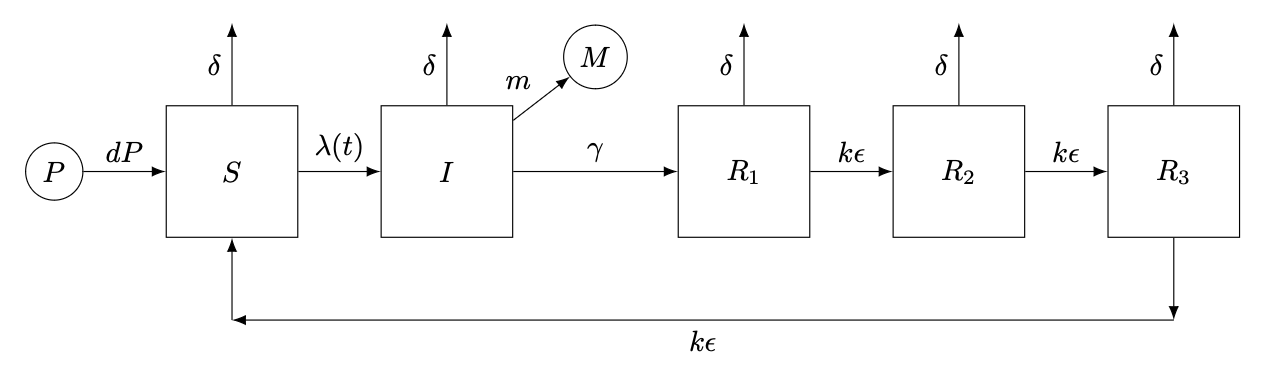
\includegraphics[width=\textwidth/2]{imgs/095/tikzcholera.png}
    \vspace*{-7mm}
    \caption{Illustration of Dhaka cholera model from \cite{king08}.}
    \label{fig:tikz-cholera}
\end{figure}

\subsection{Results}

We benchmarked IFAD against IF2 on a challenging global search problem. We re-implemented IF2 in order to do so, but chose to benchmark our results with the results of \cite{ionides15} (labeled "IF2 2015"). We note that our re-implementation ourperforms that of \cite{ionides15}, likely due to a better choice of parameters. For each method, we performed 100 searches, initialized with 100 initial starting parameter vectors drawn uniformly from the same wide bounding box used in \cite{ionides15}. We summarize our findings below. 

\kevin{Dynamically save to a tex file and load from there}

\begin{table}[h!]
\centering
\begin{tabular}{||c c c||} 
 \hline
 Method & Best Log-Likelihood & Rank \\ [0.5ex] 
 \hline\hline
     IFAD-0 & -3747.87 & 1\\
     IFAD-1 & -3748.53 & 2\\
     IF2 (Ours) & -3755.91 & 3\\
     IF2 (Warm Start) & -3759.60 & 4 \\
     IF2 2015 & -3768.63 & 5\\ 
     MOP-0 Alone & -3795.74 & 6\\
     MOP-1 Alone & -3797.38 & 7\\
 \hline
\end{tabular}
\caption{Maximum log-likelihood found by IF2, IFAD, and MOP alone. IFAD performs the best among all methods. Our implementation of IF2 outperforms that of \cite{ionides15}, but still ultimately underperforms IFAD. IFAD manages to find the MLE, matching the highest log-likelihood previously found in the \texttt{dacca()} model implemented within the \texttt{pomp} package of \cite{king16}.}
\label{table:mle}
\end{table}

\paragraph{IFAD Successfully Finds the MLE:} Previously, the MLE at a log-likelihood of $-3748.5$ was found by \cite{king16} with much effort, using many global and local IF2 searches, with the assistance of likelihood profiling. Meanwhile, \cite{ionides15} only achieve a maximum log-likelihood of $-3768.63$, while \cite{king08} only achieve a best possible estimate of $-3793.4$. Despite being initialized for a global search, IFAD manages to find the MLE over the 100 searches, as seen in Table \ref{table:mle}. This suggests that the local search and refinement that was previously necessary for finding the MLE with IF2 is \textbf{baked into} the two-stage IFAD algorithm. 


\paragraph{IFAD Outperforms Both IF2 and MOP Alone:} While IF2 quickly approaches a neighborhood of the MLE within only 40 iterations (as seen in Figure \ref{fig:scatter-optim}), performing IF2 alone ultimately fails to squeeze out the last few log-likelihood units, as no IF2 search comes within 7 log-likelihood units of the MLE (as seen in Figure \ref{fig:scatter-optim}). Conversely, when we tried gradient descent with MOP alone, we encountered many, many failed searches. This is a difficult, nonconvex, and noisy problem, and the search gets stuck in local minima and saddle points, failing to approach the MLE. 

IFAD, in comparison, manages to (1) approach the MLE quickly due to the IF2 warm-start (as seen in Figure \ref{fig:scatter-optim}) and (2) refine the coarse solution found by the warm-start with MOP gradient steps to find the MLE (as seen in Figures \ref{fig:scatter-optim} and \ref{fig:boxplot-search}. IFAD therefore successfully combines the best qualities of IFAD and MOP, outperforming either of them alone. 


\kevin{Increase size of font in legend, notch rest of font up by one point. Make figure aspect ratio to be taller than wider.}
\begin{figure}[htbp!]
    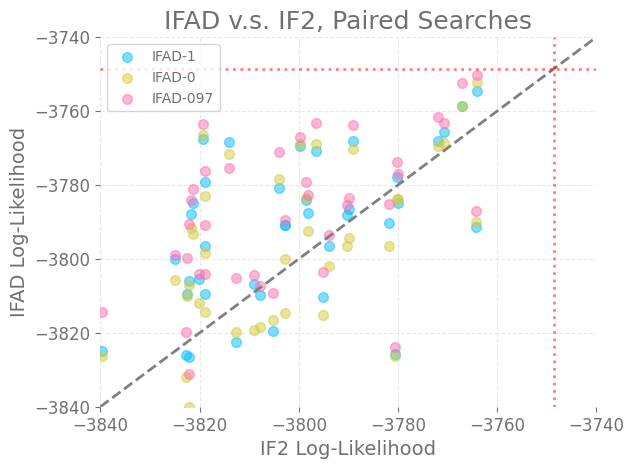
\includegraphics[width=\textwidth/\real{4.2}]{../imgs/095/pairs.png}
    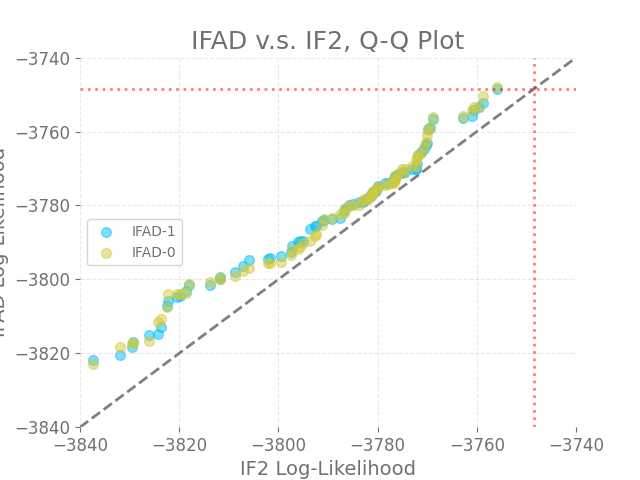
\includegraphics[width=\textwidth/\real{4.2}]{../imgs/095/qq.png}
    \caption{Scatterplots depicting the performance of IFAD against that of IF2. \textbf{Left:} Paired searches from the same starting point. Controlling for initial starting point, tuning $\alpha$ allows IFAD-$0.97$ to strictly improve on IF2, \cite{poyiadjis11}, and \cite{blei2018vsmc}, on almost every iteration. \textbf{Right:} Q-Q plot of ranked IFAD searches against ranked IF2 searches. It is clear that on average, IFAD has the edge, and manages to find the MLE while no IF2 search successfully gets within 7 log-likelihood units of it. We use a dotted red line to display the MLE in both. }
    \label{fig:scatter-optim}
\end{figure}

\kevin{Include plots of IFAD vs Poyiadjis and Naesseth only in the supplemental information}

\begin{figure}[ht]
    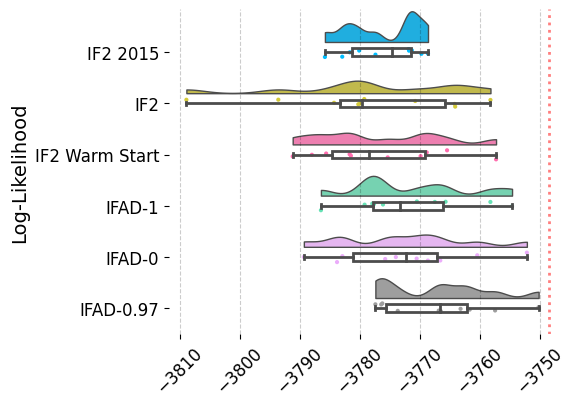
\includegraphics[width=\textwidth/\real{4.2}]{../imgs/095/boxplot.png}
    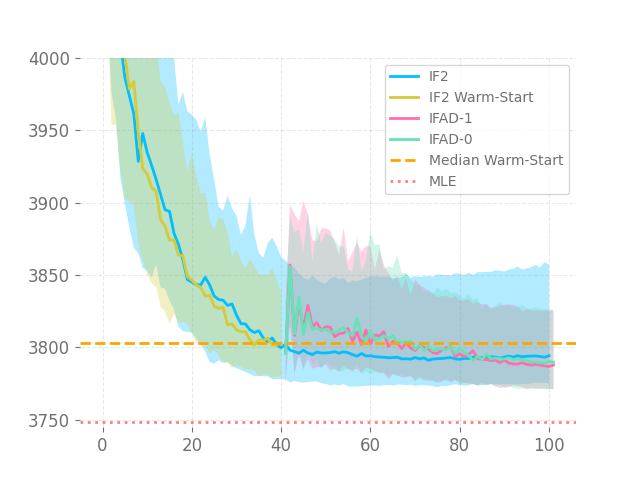
\includegraphics[width=\textwidth/\real{4.2}]{../imgs/095/optim.png}
    \caption{\textbf{Left:} Boxplot depicting the performance of IFAD and IF2 where we plot the results of the best run out of every ten runs, simulating the result of the common procedure of running a few searches and choosing the best one. IFAD outperforms all other methods, and the gradient steps improve on the warm-start given by running 40 IF2 iterations. 
    \textbf{Right:} Optimization progress of IFAD and IF2. The dashed orange line depicts the median warm-start given by running 40 IF2 iterations. While running 60 more iterations of IF2 improves upon the median warm-start, doing so ultimately underperforms IFAD -- IFAD has better tail control and successfully reaches the MLE. 
    We use a dotted red line to display the MLE.}
    \label{fig:boxplot-search}
\end{figure}


\section{Theoretical Analysis of MOP-$\alpha$}
\label{sec:thms}

Here, we will show that MOP-$\alpha$ targets the posterior and likelihood, yields the estimators of \cite{poyiadjis11, scibior21, blei2018vsmc} as special cases when differentiated, and characterize rates for its bias and variance under different choices of $\alpha$. To do so, we require the following assumptions:

\begin{enumerate}[label=(A\arabic*),itemsep=-1.2ex] 
    \item \textbf{Continuity of the Likelihood.} $\ell(\theta)$ has more than two continuous derivatives in a neighborhood $\left\{\theta: \ell(\theta)>\lambda_1\right\}$ for some $\lambda_1<\sup _{\varphi} \ell(\varphi)$. \label{assump:conti-lik}
    \item \textbf{Bounded Process Model.} There exist $\underbar{M}, \bar{M}$ such that $0 < \underbar{M} \leq f_{X_n|X_{n-1}}(x_n | x_{n-1};\theta) \leq \bar{M} < \infty$. \label{assump:bounded-process}
    \item \textbf{Bounded Measurement Model.} There exist $\underbar{G}, \bar{G}$ such that $0<\underbar{G} \leq f_{Y_n \mid X_n}\left(y_n^* \mid x_n; \theta\right) \leq \bar{G}<\infty$ and $G'(\theta)$ so $||\nabla_\theta \log f_{Y_n \mid X_n}\left(y_n^* \mid x_n; \theta\right)||_\infty \leq G'(\theta)< \infty$. \label{assump:bounded-measurement}
    \item \textbf{Bounded Gradient Estimates.} There are functions $G(\theta), H(\theta): \Theta \to [0,\infty)$ uniformly bounded by $G', H'$, so the MOP-$\alpha$ gradient and Hessian estimates at $\theta=\phi$ are almost surely bounded by $G(\theta)$ and $H(\theta)$ for all $\alpha$. \label{assump:local-bounded-derivative}
    \item \textbf{Differentiability of Density Ratios and Simulator.} The measurement density $f_{Y_n|X_n}(y_n^*|x; \theta)$ and simulator have more than two continuous derivatives in $\theta$. \label{assump:diff-meas-and-sim}
\end{enumerate}

The fact that the likelihood estimate yielded by MOP-$\alpha$ has more than two continuous derivatives in $\theta$ follows the construction of the likelihood estimate in equations \ref{eq:mop-conditional-likelihood} and \ref{eq:weighting-scheme}, as well as Assumptions \ref{assump:bounded-measurement} and \ref{assump:diff-meas-and-sim}. 

\subsection{MOP-$\alpha$ Targets the Posterior}


We show here that MOP-$\alpha$ targets the posterior and is strongly consistent for the likelihood. While the result is presented here as specific to MOP-$\alpha$, we actually prove a more general result in the supplementary material. That is, we show a strong law of large numbers for triangular arrays of particles with ``off-policy'' resampling, where we resample the particles according to an arbitrary resampling rule not necessarily in proportion to the targeted distribution of interest, to weights that encode the cumulative discrepancy between the resampling and the target distribution instead of equal weights.

\kevin{Should we just show the general result? That is, for an arbitrary set of indices $k_{n,j}$ generated in proportion to some arbitrary weights $\pi_{n,j}$ that do not necessarily sum to $1$ as the estimate is self-normalized, reweighting the particles by $w_{n,a(j)}g_{n,a(j)}/\pi_{n,a(j)}$ targets the posterior. $\pi_{n,j}$ can depend on $\{(x_{n,1:J},g_{n,1:J})\}$ as long as the resampling is carried out independently of $\{(x_{n,1:J},g_{n,1:J})\}$, conditional on $\pi_{n,1:J}$}

\begin{thm}[MOP-$\alpha$ Targets the Posterior and Likelihood]
    \label{thm:mop-targeting}
    When $\alpha=1$ or $\theta=\phi$, MOP-$\alpha$ targets the posterior and is strongly consistent for the likelihood. That is, for $\pi_n(\theta)=f_{X_{1:n}|Y_{1:n} ; \theta}$ and any measurable and bounded functional $h$ and for $\hat\lik(\theta) = \prod_{n=1}^N L_n^{A,\theta,\alpha}$ or $\prod_{n=1}^N L_n^{B,\theta,\alpha}$, it holds that
    \vspace*{-2.5mm}
    \begin{equation}
        \frac{\sum_{j=1}^J h(x_{n,j}^{A,F, \theta}) w_{n,j}^{A,F,\theta}}{\sum_{j=1}^J w_{n,j}^{A,F,\theta}} \stackrel{a.s.}{\to} E_{\pi_n(\theta)} h, \;\; \hat\lik(\theta)  \stackrel{a.s.}{\to} \lik(\theta).
    \vspace*{-2.5mm}
    \end{equation}
\end{thm}

\kevin{Write the supplement formally with Del Moral-lite language, going into full detail with the proofs and calculations.}

\begin{proof}
    We provide a proof sketch here, deferring most of the details, and discussion of the after-resampling conditional likelihood estimate $L_n^{A,\theta,\alpha}$, to the supplementary information. 
    
    When $\theta=\phi$, regardless of the value of $\alpha$, the ratio ${g_{n,j}^\theta}/{g_{n,j}^\phi}=1,$ and this reduces to the vanilla particle filter.
    
    When $\alpha=1$ and $\theta\neq\phi,$ suppose inductively that $\{(X^{F,\theta}_{n-1,j},w^{F,\theta}_{n-1,j})\}_{j=1}^J$ targets $f_{X_{n-1}|Y_{1:n-1}}(x_{n-1}|y^*_{1:n-1};\theta)$.
    It can then be shown that $\{(X^{P,\theta}_{n,j},w^{P,\theta}_{n,j})\}_{j=1}^J$ targets $f_{X_{n}|Y_{1:n-1}}(x_{n}|y^*_{1:n-1};\theta)$, that $\{(X^{P,\theta}_{n,j},w^{P,\theta}_{n,j} g^\theta_{n,j} )\}_{j=1}^J$ targets  $f_{X_{n}|Y_{1:n}}(x_{n}|y^*_{1:n};\theta)$, and that weighting the particles by $(X^{F,\theta}_{n,j},w^{F,\theta}_{n,j}) = (X^{P,\theta}_{n,a(j)}, w^{P,\theta}_{n,a(j)} g^\theta_{n,a(j)}/ g^\phi_{n,a(j)})$ where $a(\cdot)$ is the ancestor function,
    resampling with probabilities proportional to $g^\phi_{n,j}$, also targets $f_{X_{n}|Y_{1:n}}(x_{n}|y^*_{1:n};\theta)$.

    If the likelihood is estimated with the before-resampling conditional likelihoods $\hat\lik(\theta) = \prod_{n=1}^N L_n^{B,\theta,\alpha}$, the strong consistency is a direct consequence of our earlier result that $\{ \big(X^{P,\theta}_{n,j},w^{P,\theta}_{n,j}\big) \}$ targets $f_{X_{n}|Y_{1:n-1}}(x_{n}|y^*_{1:n-1};\theta)$. 
\end{proof}




\subsection{MOP-$1$ Is Consistent for the Score}

Despite showing that the MOP-$1$ gradient estimate yields the estimate of \cite{poyiadjis11, scibior21} when applied to the bootstrap filter, \cite{poyiadjis11, scibior21} use $\frac{1}{J}\sum_{j=1}^J \nabla_\theta \log f_{Y_{1:N}, X_{1:N}}\left(y_{1:N}^* , x_{1:n,j}^{A, F,\theta}; \theta\right)$ in general. The bootstrap and general estimates have different functional forms, and are not the same a-priori. As such we directly show the consistency of the MOP-$1$ gradient estimate below. 

\begin{thm}[Consistency of MOP-$1$ Gradient Estimate]
    The gradient estimate of MOP-$\alpha$ when $\alpha=1$, $\theta=\phi$ is strongly consistent for the score: $\nabla_\theta \hat\ell_J^1(\theta) \stackrel{a.s.}{\to} \nabla_\theta \ell(\theta)$ as $J \to \infty$.
    \label{thm:mop-grad-consistency}
\end{thm}
\begin{proof}
    Fix $\omega \in \Omega$, and set $\phi = \theta$, where $\theta$ is the point we wish to evaluate the gradient at. The sequence $(\nabla_\theta \hat\lik_J^1(\theta)(\omega))_{J \in \mathbb{N}}$ is uniformly bounded over all $J$, by Assumption \ref{assump:local-bounded-derivative}. Again by Assumption \ref{assump:local-bounded-derivative}, the second derivative of $\hat\lik_J^1(\theta)(\omega)|_{\theta=\theta'}$ is also bounded by $H'$ for almost every $\omega\in \Omega$ and every $\theta'\in \Theta$. So $(\nabla_\theta \hat\lik_J^1(\theta)( \omega))_{J \in \mathbb{N}}$ is uniformly Lipschitz, and therefore uniformly equicontinuous for almost every $\omega \in \Omega$.

    By Arzela-Ascoli, there is a uniformly convergent subsequence. But there is only one subsequential limit, as we can treat the gradient estimate at $\theta$ as a bounded functional of the particles by Assumption \ref{assump:local-bounded-derivative}, allowing us to apply Theorem \ref{thm:mop-targeting} to see that the sequence $(\nabla_\theta \hat\lik_J^1(\theta, \omega))_{J \in \mathbb{N}}$ converges pointwise for $\theta=\phi$ and almost every $\omega \in \Omega$. So the whole sequence must converge uniformly to $\lim_{J \to \infty} \nabla_\theta \hat\lik_J^1(\theta)(\omega).$ 
    
    With uniform convergence for the derivatives established, we can swap the limit and derivative and obtain, in conjunction with the strong consistency $\hat{\lik}_J^1(\theta, \omega) \stackrel{a.s.}{\to} \lik(\theta)$ in Theorem \ref{thm:mop-targeting}, that for almost every $\omega \in \Omega$, 
    $\lim_{J \to \infty} \nabla_\theta \hat\lik_J^1(\theta)(\omega) = \nabla_\theta \lim_{J \to \infty} \hat\lik_J^1(\theta)(\omega) = \nabla_\theta \lik(\theta).$
    The result then follows by the continuous mapping theorem. 
\end{proof}


\subsection{MOP-$\alpha$ Bias and Variance}
\begin{thm}
    \label{thm:mop-biasvar}
    When $\alpha\in(0,1)$, $\theta=\phi$, the MSE and variance of MOP-$\alpha$, where $\psi(\alpha)=(\alpha^k  + \alpha^{k+1} - \alpha)(1-\alpha)^{-1}$, are:
    \vspace*{-1ex}
    \begin{align*}
        &\E||\nabla_\theta\ell(\theta) - \nabla_\theta \hat\ell^\alpha(\theta)||_2^2 
        \\
        &\lesssim \min_{k \leq N} NpG'(\theta)^2\left(k^2J^{-1}+(1-\epsilon)^{\floor{k/(c\log(J))}}+k+\psi(\alpha)\right),\\[-1ex]
        &\text{Var}(\nabla_\theta \hat\ell^{\alpha}(\theta)) \lesssim \min_{k\leq N} NpG'(\theta)^2\left(\frac{k^2}{(1-\alpha)^2J} + \frac{16\alpha^{2k}}{(1-\alpha)^2}N\right).
        \end{align*}
\end{thm}
\kevin{Explain exactly what $\epsilon$ is here, and interpret the rates as agreeing with our intuition. Talk about the relationship between the theory and the empirical results in the bias-variance tradeoff figure above, as well as the phase transition between $Nk^2/J$ and $N^4/J$ variance with MOP-$\alpha$ and MOP-$1$, where $k$ is really a surrogate for $\alpha$ -- with more memory, you truncate less. }


We defer the proof to the supplementary material in favor of a very brief outline here. 


\kevin{Say that our framework suggests whole new classes of algorithms, as it includes Naesseth and Poyiadjis. Interpolating between them with discounting is only one way to interpolate, we can also e.g. truncate at a fixed lag. Remark that the analysis is similar for MOP-$(1,k)$ as a fixed-lag filter, with slightly better rates but a less natural interpretation. We leave empirical studies of its performance to future work. }






\section{Computational Considerations}


\subsection{Runtime}

Each iteration of IF2 amounts to one iteration of the particle filter, with $O(NJ)$ time complexity. The initial "convergence" happens fairly quickly in practice. In the case of the Dhaka cholera model of \cite{king08}, when a geometric cooling multiplier of 0.95 and initial random walk standard deviation of 0.02 is used, initial convergence happens within 40 iterations of IF2. In comparison, often 100 or 200 iterations of IF2 are used for an initial global search. \cite{ionides15}, for example, use 100 iterations with the Dhaka cholera model of \cite{king08}, while \cite{wheeler23} use 200 with Model 1 in \cite{Lee_haiticholera}. 

In line with the cheap gradient principle of \cite{kakade2019provably}, getting a gradient estimate from MOP-$\alpha$ takes no more than 6 times that of the runtime of the particle filter (in practice, the multiplier is 3.75). This therefore has $O(NJ)$ time complexity as well, obtaining a gradient estimate with runtime linear in the number of particles.

\subsection{Python Library}

Re-implementing the particle filter, simulator, and MOP-$\alpha$ in \texttt{JAX} \cite{jax} enabled us to take advantage of just-in-time compilation and GPU acceleration, even with a simulator written in Python. This led to a 16x speedup (379ms vs 6.29s on a Intel i9-13900K CPU and NVIDIA RTX3090 GPU) over the CPU-only implementation of the particle filter (with a simulator written in C++) in the \texttt{pomp} package of \cite{king16}. 

\kevin{Write about new open source library that brings pomp to python with AD. There are implementations in tfp under the jax substrate, but these are not plug and play -- they require you to supply the transition densities. }




\section{Discussion, Limitations, and Future Work}

We note that it is possible to work without a differentiable simulator, but one would then require access to the transition densities. 

Our gradient estimate can be used for variational inference to approximate the posterior distribution over parameters. 

%% \subsection*{Author Affiliations}

%% Include department, institution, and complete address, with the ZIP/postal code, for each author. Use lower case letters to match authors with institutions, as shown in the example. PNAS strongly encourages authors to supply an \href{https://orcid.org/}{ORCID identifier} for each author. Individual authors must link their ORCID account to their PNAS account at \href{http://www.pnascentral.org/}{www.pnascentral.org}. For proper authentication, authors must provide their ORCID at submission and are not permitted to add ORCIDs on proofs.

% \subsection*{Format}

% Many authors find it useful to organize their manuscripts with the following order of sections: title, author line and affiliations, keywords, abstract, significance statement, introduction, results, discussion, materials and methods, acknowledgments, and references. Other orders and headings are permitted.

%% \subsection*{Manuscript Length}

%% A standard 6-page article is approximately 4,000 words, 50 references, and 4 medium-size graphical elements (i.e., figures and tables). The preferred length of articles remains at 6 pages, but PNAS will allow articles up to a maximum of 12 pages.

%% \subsection*{References}

% %% References should be cited in numerical order as they appear in text; this will be done automatically via bibtex,

% \subsection*{Data Archival}

% PNAS must be able to archive the data essential to a published article. Where such archiving is not possible, deposition of data in public databases, such as GenBank, ArrayExpress, Protein Data Bank, Unidata, and others outlined in the \href{https://www.pnas.org/author-center/editorial-and-journal-policies#materials-and-data-availability}{Information for Authors}, is acceptable.





%% \subsection*{Digital Figures}

%% EPS, high-resolution PDF, and PowerPoint are preferred formats for figures that will be used in the main manuscript. Authors may submit PRC or U3D files for 3D images; these must be accompanied by 2D representations in TIFF, EPS, or high-resolution PDF format. Color images must be in RGB (red, green, blue) mode. Include the font files for any text.

%% Images must be provided at final size, preferably 1 column width (8.7cm). Figures wider than 1 column should be sized to 11.4cm or 17.8cm wide. Numbers, letters, and symbols should be no smaller than 6 points (2mm) and no larger than 12 points (6mm) after reduction and must be consistent.

%% Figures and tables should be labelled and referenced in the standard way using the \verb|\label{}| and \verb|\ref{}| commands.

%% Figure \ref{fig:dacca-fit} shows an example of how to insert a column-wide figure. To insert a figure wider than one column, please use the \verb|\begin{figure*}...\end{figure*}| environment. Figures wider than one column should be sized to 11.4 cm or 17.8 cm wide. Use \verb|\begin{SCfigure*}...\end{SCfigure*}| for a wide figure with side legends.


%\begin{SCfigure*}[\sidecaptionrelwidth][t!]
%\centering
%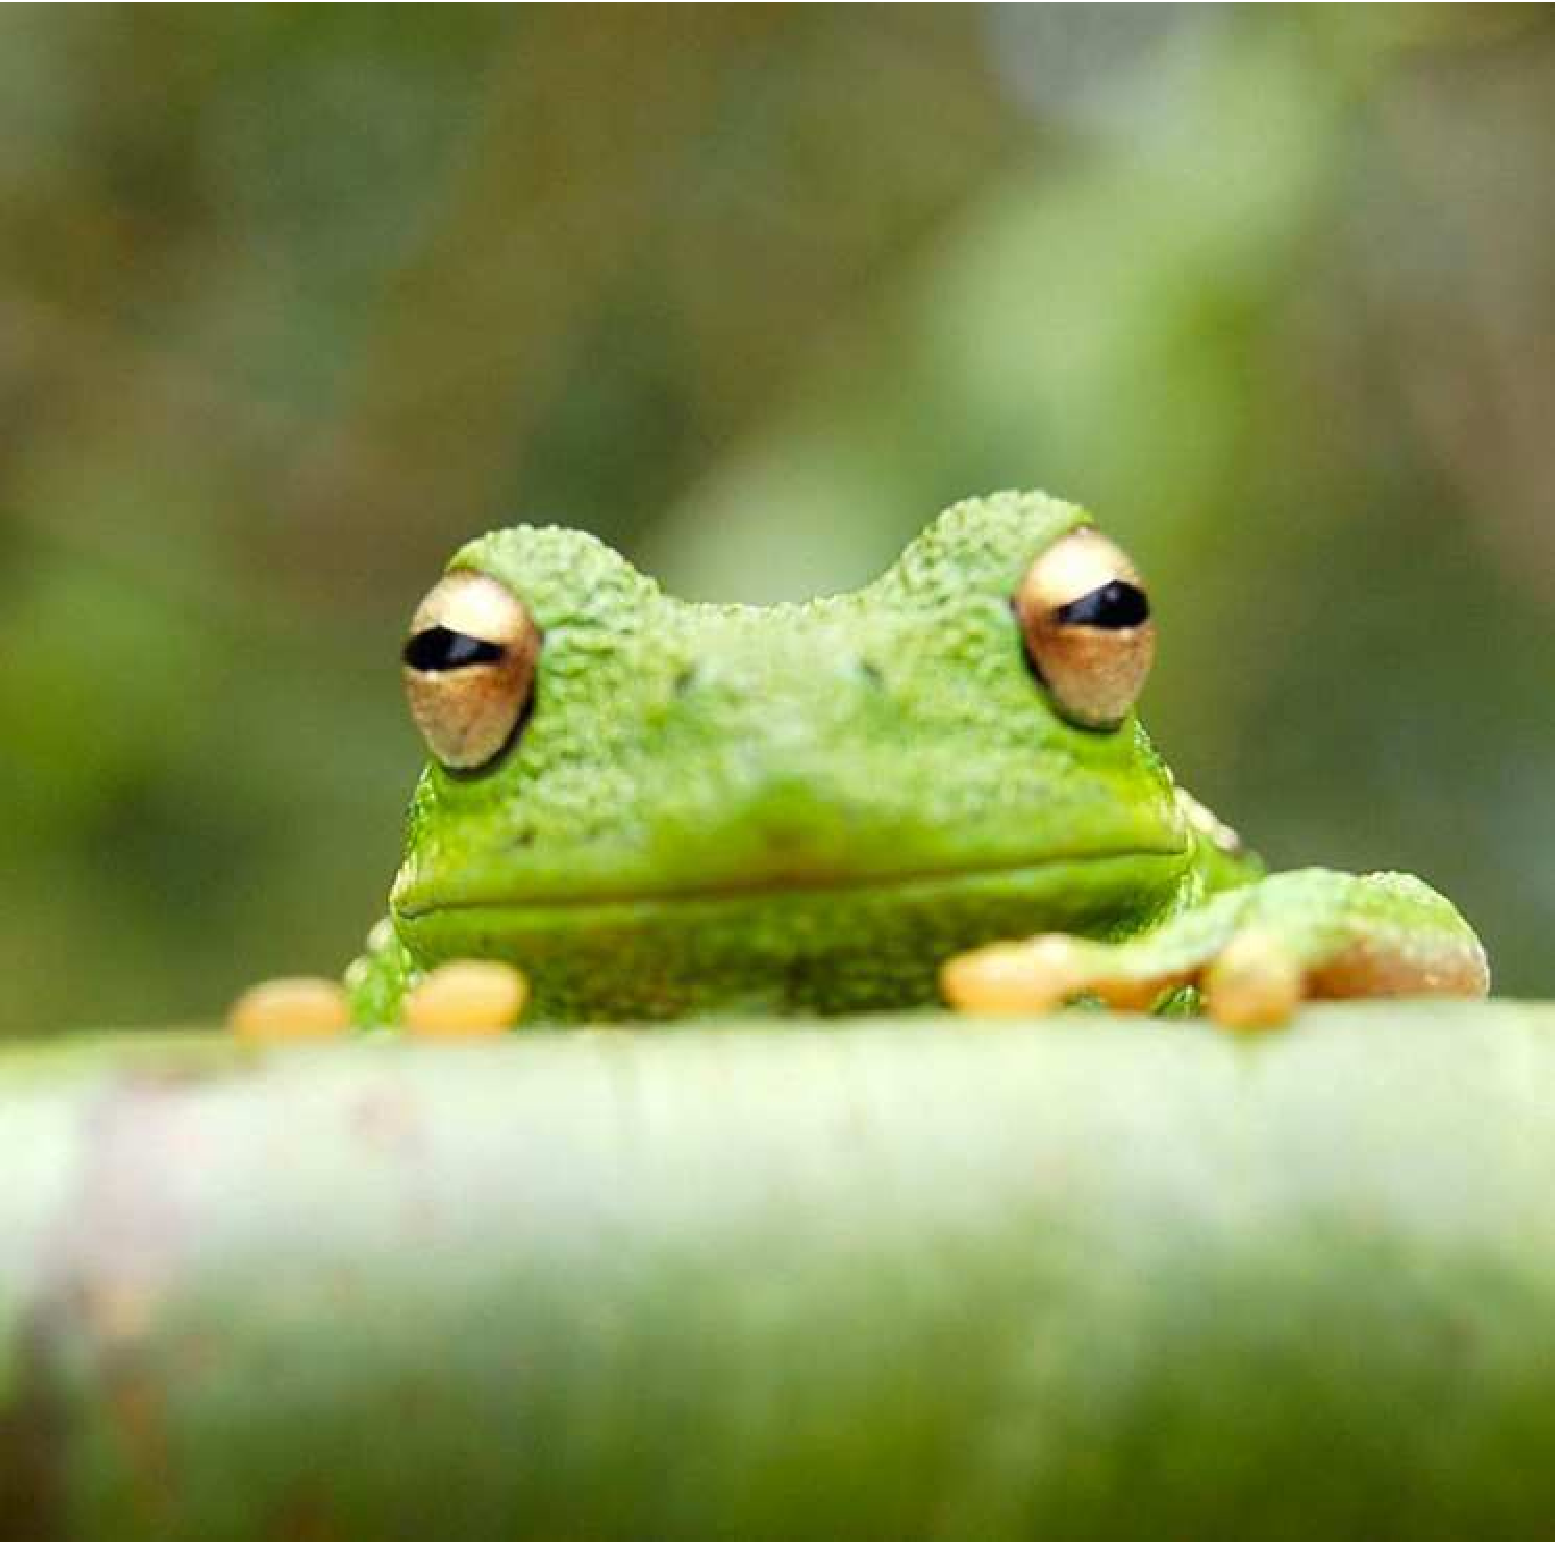
\includegraphics[width=11.4cm,height=11.4cm]{frog.pdf}
%\caption{This legend would be placed at the side of the figure, rather than below it.}\label{fig:side}
%\end{SCfigure*}


%% \subsection*{Tables}
%% Tables should be included in the main manuscript file and should not be uploaded separately.


%% \subsection*{Single column equations}

%% Authors may use 1- or 2-column equations in their article, according to their preference.

%% To allow an equation to span both columns, use the \verb|\begin{figure*}...\end{figure*}| environment mentioned above for figures.

%% Note that the use of the \verb|widetext| environment for equations is not recommended, and should not be used.

%% \begin{figure*}[bt!]
%% \begin{align*}
%% (x+y)^3&=(x+y)(x+y)^2\\
%%        &=(x+y)(x^2+2xy+y^2) \numberthis \label{eqn:example} \\
%%        &=x^3+3x^2y+3xy^3+x^3.
%% \end{align*}
%% \end{figure*}



%\subsection*{Supporting Information Appendix (SI)}

% Authors should submit SI as a single separate SI Appendix PDF file, combining all text, figures, tables, movie legends, and SI references. SI will be published as provided by the authors; it will not be edited or composed. Additional details can be found in the \href{https://www.pnas.org/authors/submitting-your-manuscript#manuscript-formatting-guidelines}{PNAS Author Center}. The PNAS Overleaf SI template can be found \href{https://www.overleaf.com/latex/templates/pnas-template-for-supplementary-information/wqfsfqwyjtsd}{here}. Refer to the SI Appendix in the manuscript at an appropriate point in the text. Number supporting figures and tables starting with S1, S2, etc.

% Authors who place detailed materials and methods in an SI Appendix must provide sufficient detail in the main text methods to enable a reader to follow the logic of the procedures and results and also must reference the SI methods. If a paper is fundamentally a study of a new method or technique, then the methods must be described completely in the main text.

% \subsubsection*{SI Datasets}

% Supply .xlsx, .csv, .txt, .rtf, or .pdf files. This file type will be published in raw format and will not be edited or composed.


\showmatmethods{} % Display the Materials and Methods section

\acknow{Please include your acknowledgments here, set in a single paragraph. Please do not include any acknowledgments in the Supporting Information, or anywhere else in the manuscript.}

\showacknow{} % Display the acknowledgments section


%\bibsplit[2]
%Use \bibsplit to split the references from the body of the text. Value "[2]" represents the number of reference in the left column (Note: Please avoid single column figures & tables on this page.)

\bibliographystyle{pnas-new}
% Bibliography
\bibliography{bib-ifad, bib-ref}

\end{document}
